\documentclass[aspectratio=169, UTF8]{ctexbeamer}
\usepackage{math214}
\usepackage{babel}
%\usepackage{enumitem}
% Then, after \begin{document}, you can begin your frames/slides

\title{\LARGE 255RC5}
\author{ Li Mingrui, Xia Yiwei, Zhang Haoran, Huang Jiayue}
\date{Summer 2024}

\definecolor{darkblue}{HTML}{6666dd} 
\colortheme{green!30!black}
%\colortheme{orange!85!black}
%\colortheme{darkblue}
%\colortheme{blue!100!black}
%\colortheme{orange!85!white!90!black}
\begin{document}

\maketitle

%\begin{frame}
 %  \frametitle{}
  %  \tableofcontents     % 生成目录
%\end{frame}


\begin{frame}{Contents}
    \begin{enumerate}
        \item \hyperlink{1}{Matrix Basic}
        \item \hyperlink{2}{Linear System and Vector Space}
        \item \hyperlink{3}{Determinant}
        \item \hyperlink{4}{Vector and Vector Function}
        \item \hyperlink{5}{Function of Several Variables}
        \item \hyperlink{6}{Tangent Planes and Linear Approximation}
        \item \hyperlink{7}{Chain Rule} 
    \end{enumerate}
       
\end{frame}

\section{Matrix Basic} 
\begin{frame}[label=1]{Notation}
  
\end{frame}

\begin{frame}{Exercises}
\begin{itemize}
    \item {1.1} Vector $v=(v_1,v_2,v_3,...v_n)^T$ satisfies $vTv=1$. Matrix $H$ satisfies $H=I_n-2XX^T$. Prove that $H$ is a symmetric matrix and $HH^T=I_n$.
    \item {1.2} Square matrix $A_(n\times n)$ satisfies $A^2+A=4I_n$. Prove that matrix $A-I_n$ is invertible and find its inverse matrix.
    \item {1.3} We have matrices $A,P and B$.
        \begin{equation*}
        A=\begin{pmatrix}
            0&-1&0\\
            1&0&0\\
            0&0&-1
        \end{pmatrix}
        \end{equation*}, $P_{3\times 3}$ is invertible, $B=P^{-1}AP$. Find $B^{2016}-2016A^2$.  
\end{itemize}    
\end{frame}

\begin{frame}
    \frametitle{Solutions}.
\end{frame}

\section{Linear System and Vector Space}


\section{Determinant}
\begin{frame}[label=3]{Definition of Determinant}
\textbf{Definition.} The determinant det : $M_{n \times n}(\mathbb{C}) \cong \underbrace{\mathbb{C}^{n} \times \cdots \times \mathbb{C}^{n}}_{n \text { times }} \rightarrow \mathbb{C}$ is the unique function satisfying
\begin{itemize}
    \item Alternating, i.e., for $v \in \mathbb{C}^{n}, \operatorname{det}\left(v_{1}, \cdots, v, \cdots, v, \cdots, v_{n}\right)=0$, or equivalently  skew-symmetric, i.e.,
    $$
\begin{aligned}
& \operatorname{det}\left(v_{1}, \ldots, v_{i-1}, v_{i}, v_{i+1}, \ldots, v_{j-1}, v_{j}, v_{j+1}, \ldots, v_{n}\right) \\
& =-\operatorname{det}\left(v_{1}, \ldots, v_{i-1}, v_{j}, v_{i+1}, \ldots, v_{j-1}, v_{i}, v_{j+1}, \ldots, v_{n}\right)
\end{aligned}
$$

\item Multilinear, i.e., for $\lambda, \mu \in \mathbb{C}, v_{i}, u \in \mathbb{C}^{n}, i=1, \cdots, n$,

$$
\begin{aligned}
& \operatorname{det}\left(v_{1}, \ldots, v_{i-1}, \lambda v_{i}+\mu u, v_{i+1}, \ldots, v_{n}\right) \\
& =\lambda \operatorname{det}\left(v_{1}, \ldots, v_{i-1}, v_{i}, v_{i+1}, \ldots, v_{n}\right) \\
& +\mu \operatorname{det}\left(v_{1}, \ldots, v_{i-1}, u, v_{i+1}, \ldots, v_{n}\right) .
\end{aligned}
$$
\item Unitary, i.e., $det I_n = 1.$
\end{itemize}

\end{frame}



\begin{frame}{Determinant Calculation}
Determinant in $\mathbb{R}^{2}$.
$$
\operatorname{det}\left(\left[\begin{array}{ll}
a & b \\
c & d
\end{array}\right]\right)=a d-b c
$$
Determinant in $\mathbb{R}^{3}$.
$$
A=\left[\begin{array}{lll}
u & v & w
\end{array}\right] \in M_{3 \times 3}(\mathbb{R}) \Rightarrow \operatorname{det} A=u \cdot(v \times w)
$$    
\end{frame}

\begin{frame}{Determinant Calculation}
    Suppose there is $n\times n$ matrix $A = (a_{ij})$
    \begin{itemize}
        \item det $A = \sum_{(m_1, ..., m_n)\in perm (n)} (sign(m_1, ..., m_n)) a_{m_1 1}...a_{m_n n}$ \\[10pt]
        where perm(n) the set off all permutations of (1,..., n). The sign of a permutation equals 1 if the natural order has been changed an even number of times and equals -1 if the natural order has been changed and odd number of times.
    \end{itemize}
    
    \begin{itemize}
        \item cofactor $A_{ij} = (-1)^{i+j}$det$(M_{ij})$ \\[10pt]
        where $M_{ij}$ is the matrix generated by deleting A's ith colume and jth row, which is called the minor of $a_{ij}$
        \\[10pt]
        det $A = \sum_{i = 1}^n a_{ij}A_{ij} = \sum_{j = 1}^n a_{ij}A_{ij}$
    \end{itemize}
\end{frame}

\begin{frame}{Properties of Determinant}
    \textbf{Properties}
\begin{itemize}
    \item $\operatorname{det}(c A)=c^{n} \operatorname{det}(A)$ for $A \in M_{n \times n}(\mathbb{C})$ and $\lambda \in \mathbb{C}$.
    \item $\operatorname{det}(A)=\operatorname{det}\left(A^{T}\right)$.
    \item $\operatorname{det}(A B)=\operatorname{det}(A) \operatorname{det}(B)$ for $A, B \in M_{n \times n}(\mathbb{C})$.
    \item If $A=\left(a_{ij} \right)$ is a triangular matrix, i.e., $a_{ij} =0$ for $i>j$ (or $i<j$ ), then 
    $$\operatorname{det}(A)=a_{11} a_{22} \cdot a_{n n}=\prod_{i=1}^{n} a_{i i}$$
\end{itemize}
\end{frame}

\section{Vector and Vector Functions}
    \subsection{Vectors} 

    \begin{frame}[label=4]{Vectors}
        \begin{block}{Vector}
            \par \textbf{Definition.} A \textbf{vector} is an object that captures a direction and a magnitude (length) in 2D/3D spaces. Geometrically, vectors are arrows in an arbitrary position in 2D/3D spaces.

            \par \textbf{Definition.} The \textbf{tip} of the vector is the end with the arrow, while the \textbf{tail} is the end without it.

            \par \textbf{Definition.} A vector drawn with its tail at the origin is called a \textbf{position vector}.
        \end{block}

        \begin{itemize}
            \item Basis of $\mathbb{R}^3$: $\bar{e}_1,\bar{e}_2,\bar{e}_3$.
            \item Resolving a vector into components: $\bar{v} = v_1 \bar{i} + v_2 \bar{j} + v_3 \bar{k}$.
            \item Magnitude: $\left| \bar{v} \right| = \sqrt{v_1^2 + v_2^2 + v_3^2}$.
            \item $n$-dimensional vector $\bar{v} = (v_1,v_2,\cdots,v_n)$. $\left| \bar{v} \right| = \sqrt{\sum\limits_{k=1}^{n}v_k^2}$.
        \end{itemize}
    \end{frame}

    \begin{frame}[t]{Properties of Vectors}
        \par Let $\bar{a}$, $\bar{b}$ and $\bar{c}$ be $n$-dimensional vectors and $\alpha,\beta$ be real numbers (scalars). Then 
        \begin{enumerate}
            \item $\bar{a} + \bar{b} = \bar{b} + \bar{a}$.
            \item $\bar{a} + (\bar{b} + \bar{c}) = (\bar{a} + \bar{b}) + \bar{c}$.
            \item $\bar{a} + \bar{0} = \bar{a}$.
            \item $\bar{a} + (-\bar{a}) = \bar{0}$.
            \item $\alpha (\bar{a} + \bar{b}) = \alpha\bar{a} + \alpha\bar{b}$.
            \item $(\alpha \beta)\bar{a} = \alpha (\beta \bar{a})$.
            \item $(\alpha + \beta)\bar{a} = \alpha \bar{a} + \beta \bar{a}$.
            \item $1 \cdot \bar{a} = \bar{a}$.
        \end{enumerate}
    \end{frame} 

    \subsection{Vector Functions}
    \begin{frame}[t]{Vector Functions}
        \begin{block}
            \par \textbf{Definition.} A \textbf{vector-valued function} pr \textbf{vector function} is a function whose domain is a subset of the reals and range is a set of vectors, \textit{i.e.}, we say that $\bar{r}$ is a \textbf{vector function} if $\bar{r}: A \to \mathbb{R}^3$ where $A \subseteq \mathbb{R}$.
        \end{block}

        \phantom{zjy}
        
        \par For $\bar{r} (t) = f(t) \bar{i} + g(t) \bar{j} + h(t) \bar{k}$, we introduce the parametric equations 
        \begin{equation*}
            x = f(t),\ y = g(t),\ z = h(t) 
        \end{equation*}

        \begin{block}{Limit of a Vector Function}
            \par \textbf{Definition.} Let $\bar{r}(t) = f(t) \bar{i} + g(t) \bar{j} + h(t) \bar{k}$ be a vector function and $a \in \mathbb{R}$. If the limits $\lim\limits_{t \to a}f(t)$, $\lim\limits_{t \to a}g(t)$ and $\lim\limits_{t \to a}h(t)$ exist, then $\lim\limits_{t \to a} \bar{r} (t)$ exists and 
            \begin{equation*}
                \lim _{t \rightarrow a} \bar{r}(t)=\left(\lim _{t \rightarrow a} f(t)\right) \bar{i}+\left(\lim _{t \rightarrow a} g(t)\right) \bar{j}+\left(\lim _{t \rightarrow a} h(t)\right) \bar{k} .
            \end{equation*}
        \end{block}
    \end{frame}

    \begin{frame}[t]{Vector Functions}
        \begin{block}{Continuity of a Vector Function}
            \par \textbf{Definition.} Let $A \subseteq \mathbb{R}$. A vector function $\bar{r}: A \to \mathbb{R}^3$ is \textbf{continuous} at a point $a \in \mathbb{R}$ if $a \in A$ and 
            \begin{equation*}
                \lim\limits_{t \to a}\bar{r} (t) = \bar{r} (a).
            \end{equation*}

            \phantom{zjy}

            \par We say that $\bar{r}: A \to \mathbb{R}^3$ is \textbf{continuous on an interval} $I$ if $\bar{r}$ is continuous at all points $a \in I$.
            \par The continuity of $\bar{r}$ is equivalent to the continuity of $f(t)$, $g(t)$ and $h(t)$.
        \end{block}
    \end{frame}

    \begin{frame}[t]{Vector Functions}
        \begin{block}{Differentiability}
            \par \textbf{Definition.} Let $A \subseteq \mathbb{R}$ and $\bar{r}: A \to \mathbb{R}^3$. Let $t \in A$. If the limit
            \begin{equation*}
                \dfrac{d \bar{r}}{dt} = \bar{r}'(t) = \lim\limits_{h \to 0} \dfrac{\bar{r}(t+h) - \bar{r}(t)}{h}
            \end{equation*}
            exists, then we say that $\bar{r}$ is \textbf{differentiable} at $t$.
        \end{block}

        \begin{block}{Criteria for Differentiability}
            \par \textbf{Theorem.} If $\bar{r} = f(t) \bar{i} + g(t) \bar{j} + h(t) \bar{k}$ where $f$, $g$ and $h$ are functions differentiable on an interval $I$, then $\bar{r}$ is differentiable at every point in $I$ and 
            \begin{equation*}
                \bar{r}'(t) = f'(t) \bar{i} + g'(t) \bar{j} + h'(t) \bar{k} .
            \end{equation*}
        \end{block}
    \end{frame}

    \begin{frame}[t]{Vector Functions}
        \begin{block}{Integration}
            \par \textbf{Definition.} Let $\bar{r}(t) = f(t) \bar{i} + g(t) \bar{j} + h(t) \bar{k}$ where $f$, $g$ and $h$ are functions that are integrable on $[a,b]$. Then
            \begin{equation*}
                \int_{a}^{b} \bar{r}(t) d t=\left(\int_{a}^{b} f(t) d t\right) \bar{i}+\left(\int_{a}^{b} g(t) d t\right) \bar{j}+\left(\int_{a}^{b} h(t) d t\right) \bar{k}
            \end{equation*}
            \begin{equation*}
                \int \bar{r}(t) d t=\left(\int f(t) d t\right) \bar{i}+\left(\int g(t) d t\right) \bar{j}+\left(\int h(t) d t\right) \bar{k}
            \end{equation*}
        \end{block}
    \end{frame}

    \begin{frame}[t]{Vector Functions}
        \par Let $\bar{r}: A \to \mathbb{R}^3$ be a vector function and $t \in A$. Let $P$ be the point described by the vector $\bar{r}(t)$.
        \begin{block}{Tangent Vector and Tangent Line}
            \par \textbf{Definition.} If $\bar{r}'(t)$ exists and $\bar{r}'(t) \neq 0$, then $\bar{r}'(t)$ is called the \textbf{tangent vector} to the curve defined by $\bar{r}$ at the point $P$.

            \phantom{zjy}
            
            \par \textbf{Definition.} The \textbf{tangent line} to the curve described by $\bar{r}$ at the point $P$ is the line that is parallel to the vector $\bar{r}'(t)$.
        \end{block}

        \par The \textbf{unit tangent vector}, sometimes denoted $\bar{T}(t)$, is the unit vector of $\bar{r}'(t)$
        \begin{equation*}
            \bar{T} (t) = \dfrac{\bar{r}'(t)}{|\bar{r}'(t)|} .
        \end{equation*}
    \end{frame}

    \begin{frame}[t]{Vector Functions}
        \par Let $\bar{u}$ and $\bar{v}$ be differentiable vector functions. Let $c \in \mathbb{R}$ and $f: \mathbb{R} \to \mathbb{R}$ be a differentiable function.
        \begin{block}{Properties of Differentiability}
            \begin{enumerate}
                \item $\dfrac{d}{dt} [\bar{u} (t) \pm \bar{v} (t)] = \bar{u}'(t) + \bar{v}'(t)$.
                \item $\dfrac{d}{dt} [c \bar{u}(t)] = c \bar{u}'(t)$.
                \item $\dfrac{d}{dt} [ f(t) \bar{u} (t)] = f'(t) \bar{u}(t) + f(t) \bar{u}'(t)$.
                \item $\dfrac{d}{dt} [\bar{u} (t) \cdot \bar{v} (t)] = \bar{u}'(t) \cdot \bar{v}(t) + \bar{u} (t) \cdot \bar{v}'(t)$.
                \item $\dfrac{d}{dt} [\bar{u} (t) \times \bar{v} (t)] = \bar{u}'(t) \times \bar{v}(t) + \bar{u} (t) \times \bar{v}'(t)$.
                \item $\dfrac{d}{dt} [\bar{u} (f(t))] = \bar{u}'(f(t)) f'(t)$ (Chain Rule).
            \end{enumerate}
        \end{block}
    \end{frame}

    \begin{frame}[t]{Vector Functions}
        \begin{block}{Property of the Tangent Vector}
            \par \textbf{Theorem.} Let $\bar{r} (t)$ be a vector function that is differentiable on an interval $I$. If for all $t \in I$, $|\bar{r} (t) |$ is constant, then for all $t \in I$, $\bar{r}(t)$ and $\bar{r}'(t)$ are perpendicular. 
        \end{block}

        \phantom{zjy}

        \par \textbf{Proof.} 
        \par Suppose that for all $t \in I$, $|\bar{r} (t)| = c$. Therefore 
        \begin{equation*}
            2\left(\bar{r}^{\prime}(t) \cdot \bar{r}(t)\right)=\frac{d}{d t}[\bar{r}(t) \cdot \bar{r}(t)]=\frac{d}{d t}\left[|\bar{r}(t)|^{2}\right]=\frac{d}{d t}\left[c^{2}\right]=0 .
        \end{equation*}
    \end{frame}


\section{Functions of Several Variables}
    \begin{frame}[label=5]{Functions of Several Variables}
        \begin{block}
            \par \textbf{Definition.} Let $n > 1$ be a natural number. A \textbf{real-valued function of $n$ independent variables} or just a \textbf{function of $n$ variables} is a function $f: D \to \mathbb{R}$ such that $D \subseteq \mathbb{R}^n$. We denote the function $f$ as 
            \begin{equation*}
                f(x_1, \cdots, x_n)
            \end{equation*}
        \end{block}
        

        
        \begin{itemize}
            \item  A real-valued function with $n > 1$ independent variables is a function that maps points in $n$-dimensional space to real numbers.
            \item  A function of two variables $f: D \to \mathbb{R}$ where $D \subseteq \mathbb{R}^2$ can be visualized in 3D space by $z = f(x,y)$. Functions of two variables often describe surfaces in $\mathbb{R}^3$.
        \end{itemize}
    \end{frame}

    \begin{frame}[t]{Functions of Several Variables}
        \begin{block}
            \par \textbf{Definition.} Let $f: D \to \mathbb{R}$ be a function of $n$ variables where $n \geq 1$. The \textbf{graph} of $f$ is the collection of points in $\mathbb{R}^{n+1}$ defined by 
            \begin{equation*}
                \{ (x_1, \cdots, x_n, y)| y = f(x_1, \cdots, x_n) \} .
            \end{equation*}
        \end{block}

        \begin{block}
            \par \textbf{Definition.} Let $f: D \to \mathbb{R}$ be a function of $n$ variables where $n \geq 1$ with independent variables $x_1, \cdots, x_n$. The function $f$ is \textbf{linear} if there exists $a_0, \cdots, a_n \in \mathbb{R}$ such that 
            \begin{equation*}
                f(x_1, \cdots, x_n) = a_0 + a_1 x_1 + \cdots + a_n x_n .
            \end{equation*}

            \par Linear functions of two variables specify planes in 3D space. 
        \end{block}
    \end{frame}

    \begin{frame}[t]{Functions of Several Variables}
        \begin{block}
            \par \textbf{Definition.} The \textbf{level curves} of a function $f$ of two variables are the curves with equations $f(x,y) = k$, where $k$ is a constant (in the range of $f$).Note that sometimes the equation will be in the form $f(x,y,z)=0$ and in these cases the equations of the level curves are $f(x,y,k)=0$.
        \end{block}
        
        \begin{figure}
            \centering 
            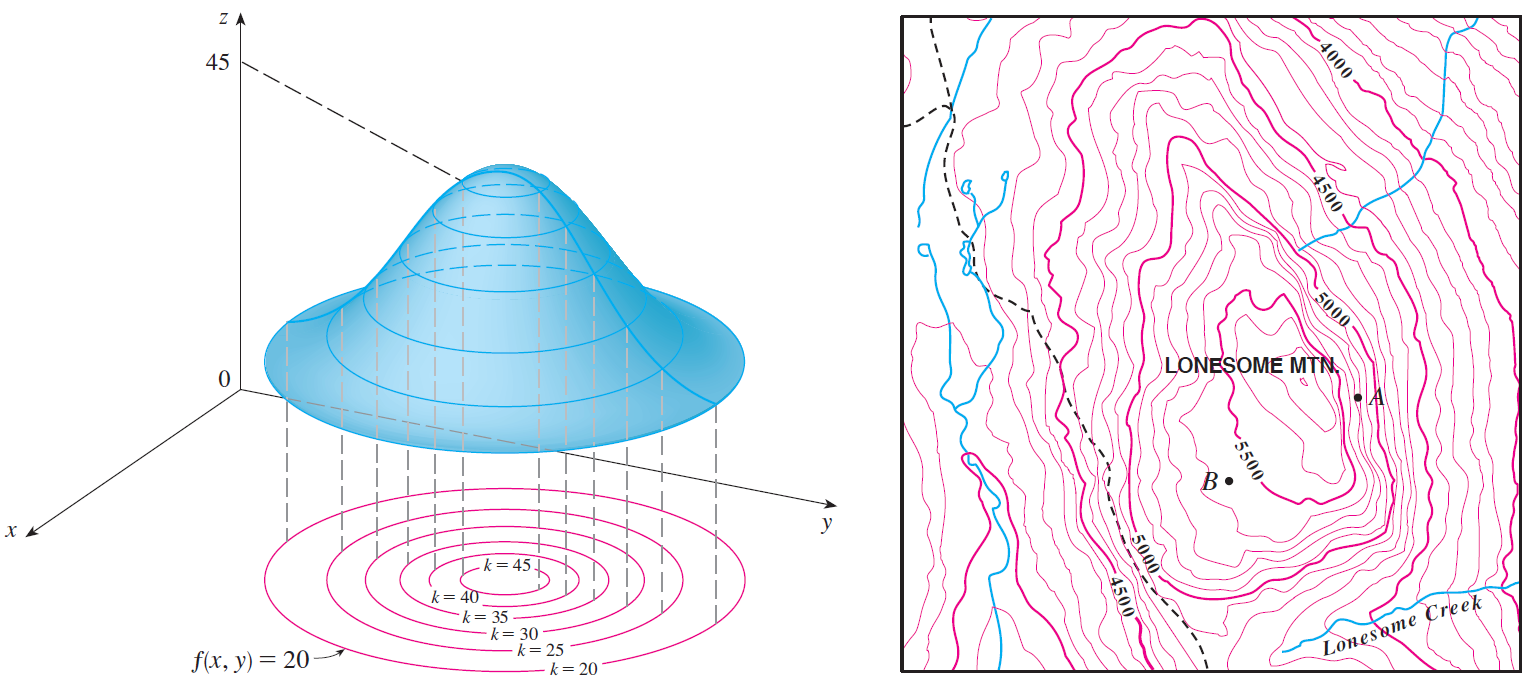
\includegraphics[width = 10cm]{f4}
            \caption{Example of Level Curves}
        \end{figure}
    \end{frame}


    \begin{frame}[t]{Limits}
        \begin{block}
            \par \textbf{Definition.} Let $f: D \to \mathbb{R}$ be a function with $D \subseteq \mathbb{R}^n$. Let $\bar{a} \in \mathbb{R}^n$ and let $L \in \mathbb{R}$. We say that the \textbf{limit} of $f$ at $\bar{x}$ approaches $\bar{a}$ is $L$ and write 
            \begin{equation*}
                \lim\limits_{\bar{x} \to \bar{a}} f(\bar{x}) = L
            \end{equation*}
            if for all $\varepsilon > 0$, there exists a $\delta > 0$ such that for all $\bar{x} \in \mathbb{R}^n$: $$||\bar{x} - \bar{a}|| < \delta \Rightarrow |f(\bar{x}) - L| < \varepsilon .$$
        \end{block}
    \end{frame}

    \begin{frame}[t]{Limits}
        \begin{figure}
            \centering 
            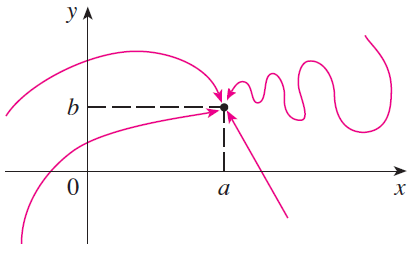
\includegraphics[width = 8cm]{f8}
            \caption{Different Directions to Approach $(a,b)$.}
        \end{figure}
    \end{frame}

    \begin{frame}[t]{Limits}
        \par Consider functions $f(x,y) = \dfrac{\sin(x^2+y^2)}{x^2+y^2}$ and $g(x,y) = \dfrac{x^2-y^2}{x^2+y^2}$.
        \begin{figure}
            \centering 
            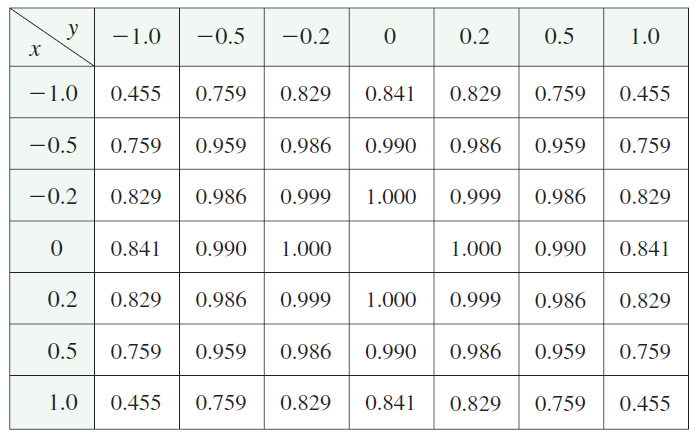
\includegraphics[width = 8cm]{f5}
            \caption{Values of $f(x,y)$.}
        \end{figure}
    \end{frame}

    \begin{frame}[t]{Limits}
        \par Consider functions $f(x,y) = \dfrac{\sin(x^2+y^2)}{x^2+y^2}$ and $g(x,y) = \dfrac{x^2-y^2}{x^2+y^2}$.
        \begin{figure}
            \centering 
            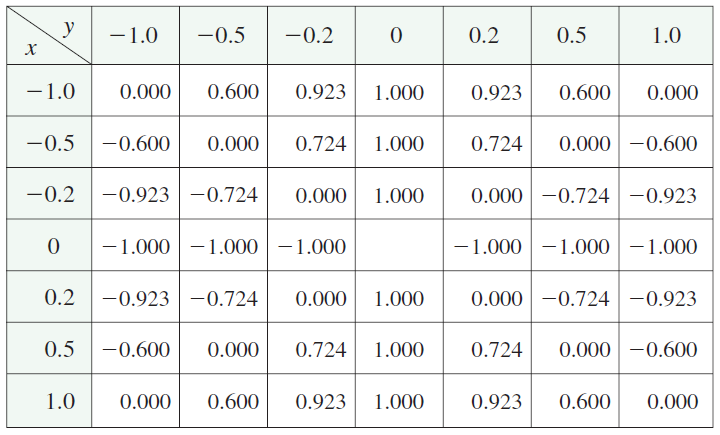
\includegraphics[width = 8cm]{f6}
            \caption{Values of $g(x,y)$.}
        \end{figure}
    \end{frame}

    \begin{frame}[t]{Limits}
        \par Here we say that 
        \begin{equation*}
            \lim _{(x, y) \rightarrow(0,0)} \frac{\sin \left(x^{2}+y^{2}\right)}{x^{2}+y^{2}}=1 \quad \text { and } \quad \lim _{(x, y) \rightarrow(0,0)} \frac{x^{2}-y^{2}}{x^{2}+y^{2}} \text{ does not exist.}
        \end{equation*}


        \begin{block}{Criteria for Limit Not Existing}
            \par Formally, if $f(x,y) \to L_1$ as $(x,y) \to (a,b)$ along a path $\mathcal{C}_1$ and $f(x,y) \to L_2$ as $f(x,y) \to (a,b)$ along a path $\mathcal{C}_2$, where $L_1 \neq L_2$, then $\lim_{(x, y) \rightarrow(0,0)} f(x,y)$ does not exist.
        \end{block}

        %\phantom{yy}

        \par \textbf{How to determine the existence of limit at the first look?}
        \par Three keys: by eye, by experience, by practice.  
    \end{frame}

    \begin{frame}[t]{Limits}
        \begin{figure}
            \centering 
            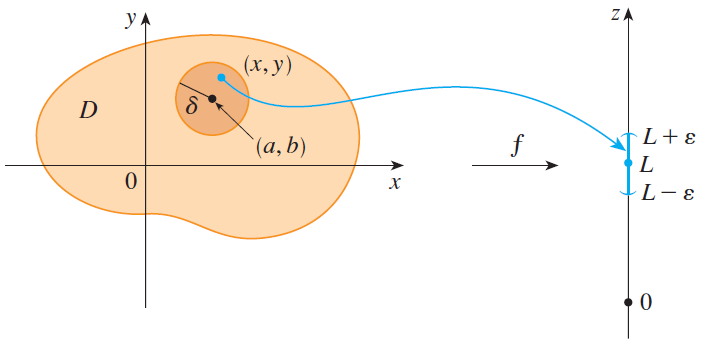
\includegraphics[width = 8cm]{f7}
            \caption{Illustration of the Definition of Limit.}
        \end{figure}
    \end{frame}

    \begin{frame}[t]{Continuity}
        \begin{block}
            \par \textbf{Definition. ($\varepsilon \delta$)} Let $f: D \to \mathbb{R}$ with $D \subseteq \mathbb{R}^n$ and let $\bar{a} \in D$. We say that $f$ is \textbf{continuous} at $\bar{a}$ if for all $\varepsilon > 0$, there exists a $\delta > 0$ such that for all $\bar{x} \in D$:
            \begin{equation*}
                || \bar{x} - \bar{a} || < \delta \Rightarrow | f(\bar{x}) - f(\bar{a}) | < \varepsilon .
            \end{equation*}

            \par \textbf{Definition. (Limit)} Let $f: D \to \mathbb{R}$ with $D \subseteq \mathbb{R}^n$ and let $\bar{a} \in D$. We say that $f$ is \textbf{continuous} at $\bar{a}$ if
            \begin{equation*}
                \lim\limits_{\bar{x} \to \bar{a}} f(\bar{x}) = f(\bar{a}) .
            \end{equation*}
        \end{block}
    \end{frame}

    \begin{frame}[t]{Continuity}
        \begin{block}
            \par \textbf{Properties of Continuity.} Let $f: D \to \mathbb{R}$ and $g: D \to \mathbb{R}$ where $D \subseteq \mathbb{R}^n$ be functions that are continuous at $\bar{a} \in D$. Let $\alpha \in \mathbb{R}$. Then 
            \begin{enumerate}
                \item $f+g$ is continuous at $\bar{a}$.
                \item $\alpha f$ is continuous at $\bar{a}$.
                \item $fg$ is continuous at $\bar{a}$.
                \item $f/g$ is continuous at $\bar{a}$ if $g(\bar{a}) \neq 0$.
            \end{enumerate}
        \end{block}
        \begin{block}
            \par \textbf{Theorem.} Let $f: D \to \mathbb{R}$ and $g: E \to \mathbb{R}$ where $D \subseteq \mathbb{R}^n$ and $E \subseteq \mathbb{R}$ be functions. Let $\bar{a} \in D$ be such that $f(\bar{a}) \in E$. If $f$ is continuous at $\bar{a}$ and $g$ is continuous at $f(\bar{a})$, then $g \circ f : D \to \mathbb{R}$ is continuous at $\bar{a}$.
        \end{block}
    \end{frame}

    \begin{frame}[t]{Continuity}
        \begin{block}
            \par \textbf{Definition.} A function $f: \mathbb{R}^n \to \mathbb{R}$ that is the sum of the terms in the form $\alpha \prod_{1 \leq i \leq n} x_i^{k_i}$ where the $x_i$'s are the independent variables, $k_i \in \mathbb{N}$ and $\alpha \in \mathbb{R}$, is called a \textbf{polynomial function of $n$ variables}.

            \par \textbf{Definition.} A function that is the quotient of polynomial functions is called a \textbf{rational function}.
        \end{block}

        \begin{block}
            \par \textbf{Theorem.} A polynomial function of $n$ variables is continuous at every point in $\mathbb{R}^n$. A rational function is continuous at every point in its domain.
        \end{block}
    \end{frame}
    
    
    \begin{frame}[t]{Continuity}
        \begin{block}{Some tips}
            1.All the standard functions that we know to be continuous are still continuous even if we are plugging in more than one variable now. We just need to watch out for division by \textbf{zero, square roots of negative numbers, logarithms of zero or negative numbers,} etc.\\
            2.Note that the idea about paths is one that we should not forget since it is a nice way to determine if a limit does not exist. If we can find two paths upon which the function approaches different values as we get near the point then we will know that the limit does not exist.
        \end{block}
        
    \end{frame}
    
    \begin{frame}{Continuity}
        \par\textbf{Exercise1.1} Determine if the following limit exist or not. If they do exist give the value of the limit.
        \begin{equation*}
            \lim_{(x,y)\to(1,1)}\frac{2x^2-xy-y^2}{x^2-y^2}
        \end{equation*}
        \par\textbf{Exercise1.2} Determine if the following limit exist or not. If they do exist give the value of the limit.
        \begin{equation*}
            \lim_{(x,y)\to(0,0)}\frac{x^2y^2}{x^4+3y^4}
        \end{equation*}
    \end{frame}

    \begin{frame}[t]{Differentiation}
        \begin{block}
            \par \textbf{Definition.} Let $f: D \to \mathbb{R}$ be a function where $D$ is an open ball of $\mathbb{R}^n$. Let $\bar{a} \in D$. The function $f$ is \textbf{differentiable} at $\bar{a}$ with \textbf{derivative} $Df(\bar{a}) \in \mathbb{R}^n$ if 
            \begin{equation*}
                \dfrac{|| f(\bar{a} + \bar{h}) - f(\bar{a}) - D f(\bar{a}) \cdot \bar{h}||}{||\bar{h}||} \to 0\ \text{as} \ \bar{h} \to \bar{0} .
            \end{equation*}
        \end{block}


        \par The derivative of the function $f$ gives the best linear approximation of $f$ at the point $\bar{a}$.

        \par The derivative of $f$ of $n$ variables is an $n$-dimensional \textbf{vector}!

        \begin{block}
            \par \textbf{Properties of Differentiation.} Let $f: D \to \mathbb{R}$ and $g: D \to \mathbb{R}$ where $D$ is an open ball of $\mathbb{R}^n$ be functions that are differentiable at $\bar{a} \in D$. Let $\alpha \in \mathbb{R}$. Then 
            \begin{enumerate}
                \item $f + g$ is differentiable at $\bar{a}$ with $D(f+g) (\bar{a}) = Df(\bar{a}) + Dg (\bar{a})$.
                \item $\alpha f$ is differentiable at $\bar{a}$ with $D(\alpha f) (\bar{a}) = \alpha D f(\bar{a})$.
            \end{enumerate}
        \end{block}
    \end{frame}

    \begin{frame}[t]{Partial Derivatives}
        \begin{block}
            \par \textbf{Definition.} Let $f: D \to \mathbb{R}$ where $D$ is an open ball of $\mathbb{R}^n$ be a function $f(x_1, \cdots, x_n)$ that is differentiable at $\bar{a} = (a_1, \cdots, a_n) \in D$. If 
            \begin{equation*}
                D f(\bar{a})=\left(\begin{array}{c}
                \alpha_{1} \\
                \vdots \\
                \alpha_{n}
                \end{array}\right)
            \end{equation*}
            then we call $\alpha_i$ the \textbf{partial derivative of $f$ with respect to $x_i$ at $\bar{a}$} and we write
            \begin{equation*}
                \left. \dfrac{\partial f}{\partial x_i} \right|_{\bar{a}} \ \text{or} \ f_{x_i} (\bar{a}) .
            \end{equation*}
        \end{block}
    \end{frame}

    \begin{frame}[t]{Partial Derivatives}
        \par \textbf{Geometric Interpretation.} For functions of two variables $f(x,y)$ we can interpret the partial derivatives geometrically. Let $(a,b,c)$ be a point such that $c = f(a,b)$ and $\mathcal{C}_1$ be the curve that is obtained by intersecting the graph $z = f(x,y)$ with the plane $y = b$ and $\mathcal{C}_2$ be the curve that is obtained by intersecting the graph $z = f(x,y)$ with the plane $x = a$. Then 
        \begin{enumerate}
            \item The partial derivative $f_x (a,b) = \lim\limits_{h \to 0} \dfrac{f(a+h,b) - f(a,b)}{h}$ is the slope of the tangent line of $\mathcal{C}_1$ in the plane $y = b$.
            \item The partial derivative $f_y (a,b) = \lim\limits_{h \to 0} \dfrac{f(a,b+h) - f(a,b)}{h}$ is the slope of the tangent line of $\mathcal{C}_2$ in the plane $x = a$.
        \end{enumerate}
    \end{frame}

    \begin{frame}[t]{Partial Derivatives}
        \begin{figure}
            \centering 
            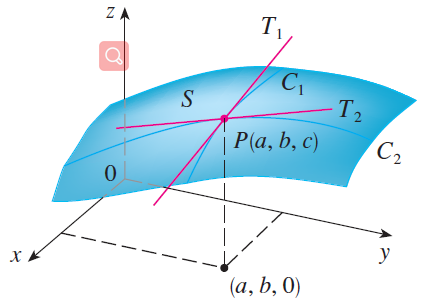
\includegraphics[width = 7cm]{f9.png}
            \caption{Geometric Interpretation of Partial Derivative.}
        \end{figure}
    \end{frame}
    
    \begin{frame}[t]{First order partial derivatives}
        \par \textbf{Exercise 2.1}  Find all of the first order partial derivatives for the following functions.
        \begin{equation*}
            w = x^2y - 10y^2z^3 + 43x - 7tan(4y)
        \end{equation*}
        \begin{equation*}
             f(x,y) = cos(\frac{4}{x})e^{x^2y-5y^3}
        \end{equation*}
        \par \textbf{Exercise2.2} Find $\frac{\partial z}{\partial x}$and $\frac{\partial z}{\partial y}$for each of the following function.
        \begin{equation*}
            x^3z^2 - 5xy^5z = x^2 + y^3
        \end{equation*}
           
    \end{frame}

    \begin{frame}[t]{Higher Partial Derivatives}
        \begin{block}
            \par \textbf{Definition.} Let $f: D \to \mathbb{R}$ where $D$ is an open ball of $\mathbb{R}^n$ be a function $f(x_1,\cdots, x_n)$ that is differentiable. If the partial derivative $f_{x_i} (x_1, \cdots, x_n)$ is differentiable, then we can find the partial derivative of it w.r.t one of the independent variables $x_j$. A partial derivative of a partial derivative is called a \textbf{second order  partial derivative}. We write 
            \begin{equation*}
                \dfrac{\partial^2 f}{\partial x_i \partial x_j} \ \text{or} \ f_{x_1x_j} (x_1, \cdots, x_n)
            \end{equation*}
            for the partial derivative of $f_{x_i} (x_1, \cdots, x_n)$ w.r.t the variable $x_j$. It becomes $\frac{\partial^2 f}{\partial x_i^2}$ when we take the partial derivative twice with respect to the same variable. 
        \end{block}
    \end{frame}
    


    \begin{frame}[t]{Higher Partial Derivatives}
        \begin{block}
            \par \textbf{Theorem. (Clairaut Theorem)} Let $f: D \to \mathbb{R}$ where $D$ is an open ball of $\mathbb{R}^2$ be a function $f(x_1, x_2)$ and let $(a,b) \in D$. If $f_{x_1x_2}$ and $f_{x_2x_1}$ are both continuous on $D$, then 
            \begin{equation*}
                f_{x_1x_2} (a,b) = f_{x_2x_1} (a,b).
            \end{equation*}
        \end{block}

        \begin{block}{Differentiable: Another Perspective}
            \par \textbf{Definition.} If $z = f(x,y)$, then $f$ is \textbf{differentiable} at $(a,b)$ if $\Delta z$ can be expressed in the form 
            \begin{equation*}
                \Delta z = f_x(a,b) \Delta x + f_y(a,b) \Delta y ++ \varepsilon_1 \Delta x + \varepsilon_2 \Delta y,
            \end{equation*}
            where $\varepsilon_1$ and $\varepsilon_2 \to 0$ as $(\Delta x, \Delta y) \to (0,0)$.

            \par \textbf{Theorem.} If the partial derivatives $f_x$ and $f_y$ exist near $(a,b)$ and are continuous at $(a,b)$, then $f$ is differentiable at $(a,b)$.
        \end{block}
    \end{frame}

    \begin{frame}[t]{Differential}
        \begin{block}
            \par \textbf{Theorem.} Let $f: D \to \mathbb{R}$ where $D$ is an open ball of $\mathbb{R}^n$ be a function $f(x_1,\cdots, x_n)$. If for all $1 \leq i \leq n$, $\frac{\partial f}{\partial x_i}$ exists and is continuous on $D$, then 
            \begin{equation*}
                \Delta f = f_{x_1} (\bar{x}) \Delta x_1 + \cdots + f_{x_n} (\bar{x}) \Delta x_n + \varepsilon_1 \Delta x_1 + \cdots + \varepsilon_n \Delta x_n.
            \end{equation*}
            where $\varepsilon_i \to 0$, $i = 1, \cdots, n$ as $(\Delta x_1, \cdots, \Delta x_n) \to \bar{0}$.
        \end{block}
        \begin{block}
            \par \textbf{Definition.} The \textbf{total differential} of a function $f:D \subset \mathbb{R}^n \to \mathbb{R}$ is 
            \begin{equation*}
                df = f_{x_1} (\bar{x}) d x_1 + \cdots + f_{x_n} (\bar{x}) d x_n
            \end{equation*}
            where $dx_1 = \Delta x_1, \cdots dx_n = \Delta x_n$. 
        \end{block}
    \end{frame}
    
    \begin{frame}[t]{Higher Partial Derivatives}
        \par \textbf{Exercise 2.3} Find all the second order derivatives for 
        \begin{equation*}
            f(x,y) = cos(2x) - x^2e^{5y} + 3y^2
        \end{equation*}
        \par \textbf{Exercise 2.4} Find $f_{xxyzz}$ for f(x,y,z) = $z^3y^2ln(x)$
    \end{frame}
    
    \begin{frame}{Differential}
        \begin{figure}
            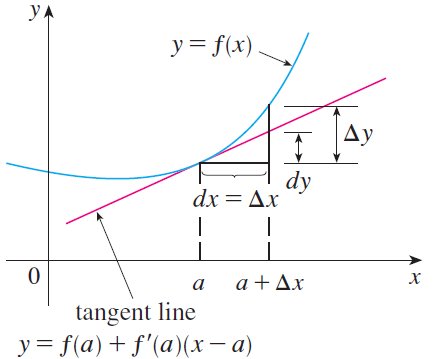
\includegraphics[width = 7cm]{f10}
            \caption{Differential $dy$ of a Single Variate Function $y = f(x)$.}
        \end{figure}
    \end{frame}


    \begin{frame}{Differential}
        \begin{figure}
            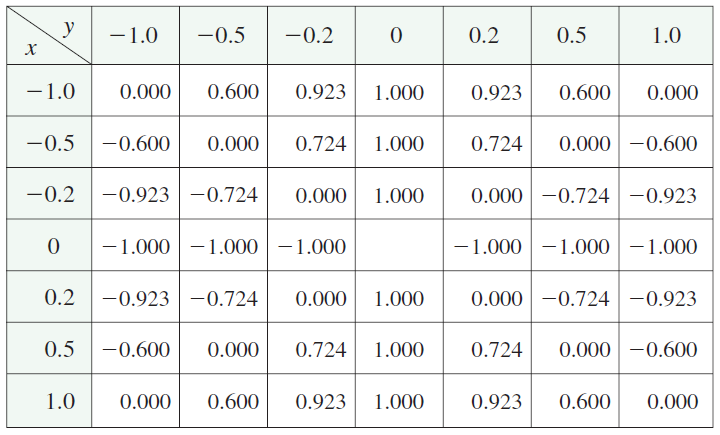
\includegraphics[width = 10cm]{f6}
            \caption{Total Differential $dz$ of Multivariate Function $z = f(x,y)$.}
        \end{figure}
    \end{frame}

\section{Tangent Planes and Linear Approximation}
    \begin{frame}[label=6]{Tangent Planes}
        \par The equation of the tangent plane of $f(x,y)$ at $(a,b)$ is 
        \begin{equation*}
            z - f(a,b) = f_x (a,b) (x-a) + f_y (a,b) (y-b) \leftarrow \text{linear approximation!}
        \end{equation*}
        \phantom{zjy}

        \par (Recall how we obtain the equation of the tangent line of a function $f(x)$ in VV156.
        
        \phantom{zjy}
    
        \par Linear Approximation: Important in Engineering.\\
        \par \textbf{Example} Find the equation of the tangent plane to z = ln(2x+y) at (-1,3)
    \end{frame}

    \begin{frame}{Tangent Planes}
        \begin{figure}
            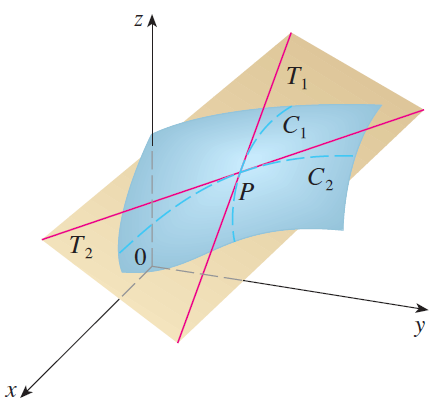
\includegraphics[width = 6cm]{f12}
            \caption{Example of Tangent Plane.}
        \end{figure}
    \end{frame}

    \begin{frame}{Linear Approximation}
        \begin{figure}
            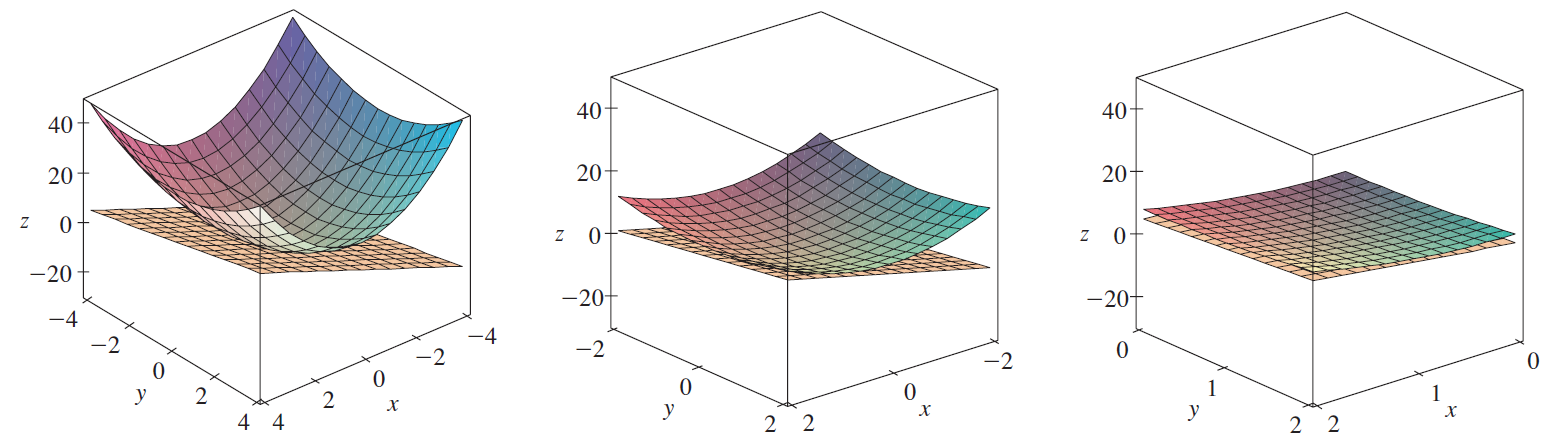
\includegraphics[width = 13cm]{f13}
            \caption{The Surface $z = 2x^2+y^2$ Appears to Coincide with its Tangent Plane.}
        \end{figure}
    \end{frame}

    \begin{frame}{Linear Approximation}
        \begin{figure}
            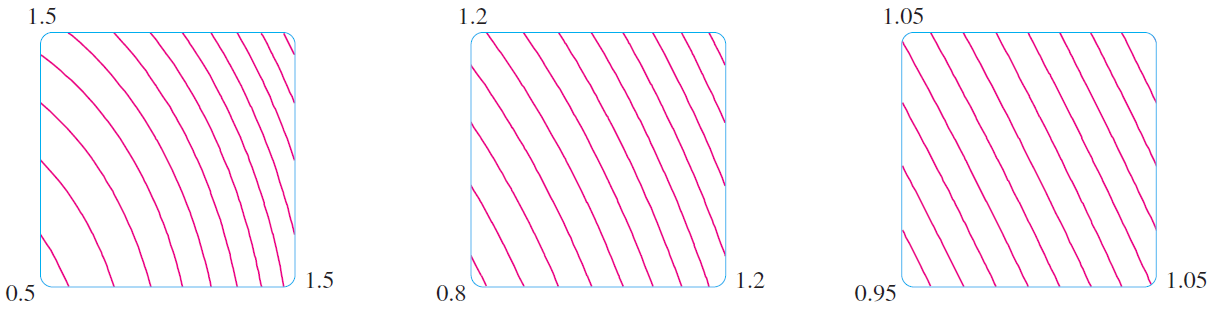
\includegraphics[width = 13cm]{f14}
            \caption{The Contour Map of $f(x,y) = 2x^2 + y^2$.}
        \end{figure}
    \end{frame}

\section{Chain Rule}
    \begin{frame}[label=7]{Chain Rule}
        \begin{block}{Chain Rule: General Version}
            \par \textbf{Theorem.} Let $u$ be a differentiable function of $n$ variables $x_1, \cdots, x_n$ such that for all $1 \leq i \leq n$, $x_i$ is a differentiable function of $m$ variables $t_1, \cdots, t_m$. Then $u$ is a function of $t_1, \cdots, t_m$ and for all $1 \leq j \leq m$, 
            \begin{equation*}
                \dfrac{\partial u}{\partial t_j} = \sum\limits_{1 \leq i \leq n} \dfrac{\partial u}{\partial x_i} \dfrac{\partial x_i}{\partial t_j}.
            \end{equation*}
        \end{block}
    \end{frame}

    \begin{frame}[t]{Chain Rule}
        \begin{block}{Chain Rule I}
            \par \textbf{Theorem.} Let $x = g(t)$ and $y = h(t)$ be functions that are differentiable on an interval $I$. Let $z = f(x,y)$ be a function that is differentiable at the points with $x$-coordinate in the range of $g$ restricted to $I$, and $y$-coordinates in the range of $h$ restricted to $I$. Then $f(x,y)$ is differentiable with respect to $t$ on the interval $I$ and 
            \begin{equation*}
                \dfrac{df}{dt} = \dfrac{\partial f}{\partial x} \dfrac{dx}{dt} + \dfrac{\partial f}{\partial y} \dfrac{dy}{dt} .
            \end{equation*}
        \end{block}
        \par \textbf{Exercise2.5} Find $\frac{dz}{dt}$ for $z = xe^{xy}, x = t^2, y = t^{-1}$
    \end{frame}

    \begin{frame}[t]{Chain Rule}
        \begin{block}{Chain Rule II}
            \par \textbf{Theorem.} Suppose that $z =f(x,y)$ is a differentiable function of $x$ and $y$ where $x = g(s,t)$ and $y = h(s,t)$ are differentiable functions. Then 
            \begin{equation*}
                \begin{aligned}
                    \dfrac{\partial z}{\partial s} &= \dfrac{\partial z}{\partial x} \dfrac{\partial x}{\partial s} + \dfrac{\partial z}{\partial y} \dfrac{\partial y}{\partial s} ,\\
                    \dfrac{\partial z}{\partial t} &= \dfrac{\partial z}{\partial x} \dfrac{\partial x}{\partial s} + \dfrac{\partial z}{\partial y} \dfrac{\partial y}{\partial s} .
                \end{aligned}
            \end{equation*}
        \end{block}
        \par \textbf{Exercise 2.6} Find $\dfrac{\partial z}{\partial s}$ and $\dfrac{\partial z}{\partial t}$ for $z = e^{2r}sin(3\theta), r = st - t^2, \theta = \sqrt{s^2+t^2}$
    \end{frame}

    \begin{frame}[t]{Implicit Differentiation}
        \par Assume that an equation $F(x,y) = 0$ defines $y$ implicitly as a differentiable function of $x$. If $F(x,y)$ is differentiable, then the chain rule tells us that 
        \begin{equation*}
            \dfrac{\partial F}{\partial x} \dfrac{d x}{d x} + \dfrac{\partial F}{\partial y} \dfrac{d y}{d x} = 0.
        \end{equation*}
        \par Therefore, if $\frac{\partial F}{\partial y} \neq 0$, then 
        \begin{equation*}
            \dfrac{dy}{dx} = - \dfrac{F_x}{F_y} .
        \end{equation*}
        \par Similarly, if $F(x,y,z) = 0$, we have 
        \begin{equation*}
            \dfrac{\partial F}{\partial x} \dfrac{\partial x}{\partial x} + \dfrac{\partial F}{\partial y} \dfrac{\partial y}{\partial x} + \dfrac{\partial F}{\partial z} \dfrac{\partial z}{\partial x} = 0.
        \end{equation*}
    \end{frame}
    
    \begin{frame}[t]{Jacobian Matrix}
        \begin{block}
            \par \textbf{Definition.} Suppose $F:\mathbb{R}^n\rightarrow\mathbb{R}^m$ is a function that maps from an n-dimensional space to an m-dimensional space. This function consists of $m$ functions: $f_1(x_1,x_2,\cdots, x_n),\cdots,f_m(x_1,x_2,\cdots, x_n)$. Then the Jacobian matrix is:
        \begin{equation*}
DF(x) = 
	\begin{bmatrix}
		\vspace{1.5ex}
		\dfrac{\partial f_1}{\partial x_1} & \dfrac{\partial f_1}{\partial x_2}  & \cdots & \dfrac{\partial f_1}{\partial x_n}\\ 
		\vspace{1.5ex}
		\dfrac{\partial f_2}{\partial x_1} & \dfrac{\partial f_2}{\partial x_2}  & \cdots & \dfrac{\partial f_2}{\partial x_n}\\
		\vspace{1.5ex}
		\vdots                             & \vdots                              & \vdots & \vdots                            \\
		\vspace{1.5ex}
		\dfrac{\partial f_m}{\partial x_1} & \dfrac{\partial f_m}{\partial x_2}  & \cdots & \dfrac{\partial f_m}{\partial x_n}
	\end{bmatrix}
\end{equation*}

        \end{block}

    \end{frame}

    \begin{frame}{Jacobian Matrix}
        \begin{block}
            \par \textbf{Properties of Differentiation.} Let $f: D \to \mathbb{R}$ and $g: D \to \mathbb{R}$ where $D$ is an open ball of $\mathbb{R}^n$ be functions that are differentiable at $\bar{a} \in D$. Let $\alpha \in \mathbb{R}$. Then 
            \begin{enumerate}
                \item $f + g$ is differentiable at $\bar{a}$ with $D(f+g) (\bar{a}) = Df(\bar{a}) + Dg (\bar{a})$.
                \item $\alpha f$ is differentiable at $\bar{a}$ with $D(\alpha f) (\bar{a}) = \alpha D f(\bar{a})$.
                \item $D(fg) (\bar{a}) = g (\bar{a})Df(\bar{a}) + f(\bar{a})Dg (\bar{a})$.
                \item $D(f/g) (\bar{a}) = \frac{g (\bar{a})Df(\bar{a}) - f(\bar{a})Dg (\bar{a})}{g (\bar{a})^2}$
            \end{enumerate}
        \end{block}

        \par The Jacobian matrix gives the best linear approximation of $F$ at the point $x$, when $x$ is close to $p$.
        $$F(x) \approx F(p) + DF(p)\cdot (x-p)$$
    \end{frame}
    
\end{document}